% !TeX program = pdflatex
% !TeX root = FCLoopTensorReduce.tex

\documentclass[../FeynCalcManual.tex]{subfiles}
\begin{document}
\hypertarget{fclooptensorreduce}{
\section{FCLoopTensorReduce}\label{fclooptensorreduce}\index{FCLoopTensorReduce}}

\texttt{FCLoopTensorReduce[\allowbreak{}exp,\ \allowbreak{}topos]}
performs tensor reduction for the numerators of multi-loop integrals
present in \texttt{exp}. Notice that \texttt{exp} is expected to be the
output of \texttt{FCLoopFindTopologies} where all loop integrals have
been written as
\texttt{fun[\allowbreak{}num,\ \allowbreak{}GLI[\allowbreak{}...]]} with
\texttt{num} being the numerator to be acted upon.

The reduction is done only for loop momenta contracted with Dirac
matrices, polarization vectors or Levi-Civita tensors. Scalar products
with external momenta are left untouched. The goal is to rewrite
everything in terms of scalar products involving only loop momenta and
external momenta appearing in the given topology. These quantities can
be then rewritten in terms of inverse propagators (\texttt{GLI}s with
negative indices), so that the complete dependence on loop momenta will
go into the \texttt{GLI}s.

Unlike \texttt{FCMultiLoopTID}, this function does not perform any
partial fractioning or shifts in the loop momenta.

The default value for \texttt{fun} is FCGV{[}``GLIProduct''{]} set by
the option \texttt{Head}

\subsection{See also}

\hyperlink{toc}{Overview},
\hyperlink{fcloopfindtopologies}{FCLoopFindTopologies}.

\subsection{Examples}

1-loop tadpole topology

\begin{Shaded}
\begin{Highlighting}[]
\NormalTok{topo1 }\ExtensionTok{=}\NormalTok{ FCTopology}\OperatorTok{[}\StringTok{"tad1l"}\OperatorTok{,} \OperatorTok{\{}\NormalTok{SFAD}\OperatorTok{[\{}\FunctionTok{q}\OperatorTok{,} \FunctionTok{m}\SpecialCharTok{\^{}}\DecValTok{2}\OperatorTok{\}]\},} \OperatorTok{\{}\FunctionTok{q}\OperatorTok{\},} \OperatorTok{\{\},} \OperatorTok{\{\},} \OperatorTok{\{\}]}
\end{Highlighting}
\end{Shaded}

\begin{dmath*}\breakingcomma
\text{FCTopology}\left(\text{tad1l},\left\{\frac{1}{(q^2-m^2+i \eta )}\right\},\{q\},\{\},\{\},\{\}\right)
\end{dmath*}

\begin{Shaded}
\begin{Highlighting}[]
\NormalTok{amp1 }\ExtensionTok{=}\NormalTok{ FCGV}\OperatorTok{[}\StringTok{"GLIProduct"}\OperatorTok{][}\NormalTok{GSD}\OperatorTok{[}\FunctionTok{q}\OperatorTok{]}\NormalTok{ . GAD}\OperatorTok{[}\SpecialCharTok{\textbackslash{}}\OperatorTok{[}\NormalTok{Mu}\OperatorTok{]]}\NormalTok{ . GSD}\OperatorTok{[}\FunctionTok{q}\OperatorTok{],}\NormalTok{ GLI}\OperatorTok{[}\StringTok{"tad1l"}\OperatorTok{,} \OperatorTok{\{}\DecValTok{1}\OperatorTok{\}]]}
\end{Highlighting}
\end{Shaded}

\begin{dmath*}\breakingcomma
\text{FCGV}(\text{GLIProduct})\left((\gamma \cdot q).\gamma ^{\mu }.(\gamma \cdot q),G^{\text{tad1l}}(1)\right)
\end{dmath*}

\begin{Shaded}
\begin{Highlighting}[]
\NormalTok{amp1Red }\ExtensionTok{=}\NormalTok{ FCLoopTensorReduce}\OperatorTok{[}\NormalTok{amp1}\OperatorTok{,} \OperatorTok{\{}\NormalTok{topo1}\OperatorTok{\}]}
\end{Highlighting}
\end{Shaded}

\begin{dmath*}\breakingcomma
\text{FCGV}(\text{GLIProduct})\left(\frac{(2-D) q^2 \gamma ^{\mu }}{D},G^{\text{tad1l}}(1)\right)
\end{dmath*}

\begin{Shaded}
\begin{Highlighting}[]
\NormalTok{topo2 }\ExtensionTok{=}\NormalTok{ FCTopology}\OperatorTok{[}\NormalTok{prop1l}\OperatorTok{,} \OperatorTok{\{}\NormalTok{SFAD}\OperatorTok{[\{}\FunctionTok{q}\OperatorTok{,} \FunctionTok{m}\SpecialCharTok{\^{}}\DecValTok{2}\OperatorTok{\}],}\NormalTok{ SFAD}\OperatorTok{[\{}\FunctionTok{q} \SpecialCharTok{{-}} \FunctionTok{p}\OperatorTok{,} \FunctionTok{m}\SpecialCharTok{\^{}}\DecValTok{2}\OperatorTok{\}]\},} \OperatorTok{\{}\FunctionTok{q}\OperatorTok{\},} \OperatorTok{\{}\FunctionTok{p}\OperatorTok{\},} \OperatorTok{\{\},} \OperatorTok{\{\}]}
\end{Highlighting}
\end{Shaded}

\begin{dmath*}\breakingcomma
\text{FCTopology}\left(\text{prop1l},\left\{\frac{1}{(q^2-m^2+i \eta )},\frac{1}{((q-p)^2-m^2+i \eta )}\right\},\{q\},\{p\},\{\},\{\}\right)
\end{dmath*}

1-loop self-energy topology

\begin{Shaded}
\begin{Highlighting}[]
\NormalTok{amp2 }\ExtensionTok{=}\NormalTok{ gliProduct}\OperatorTok{[}\NormalTok{GSD}\OperatorTok{[}\FunctionTok{q}\OperatorTok{]}\NormalTok{ . GAD}\OperatorTok{[}\SpecialCharTok{\textbackslash{}}\OperatorTok{[}\NormalTok{Mu}\OperatorTok{]]}\NormalTok{ . GSD}\OperatorTok{[}\FunctionTok{q}\OperatorTok{],}\NormalTok{ GLI}\OperatorTok{[}\NormalTok{prop1l}\OperatorTok{,} \OperatorTok{\{}\DecValTok{1}\OperatorTok{,} \DecValTok{2}\OperatorTok{\}]]}
\end{Highlighting}
\end{Shaded}

\begin{dmath*}\breakingcomma
\text{gliProduct}\left((\gamma \cdot q).\gamma ^{\mu }.(\gamma \cdot q),G^{\text{prop1l}}(1,2)\right)
\end{dmath*}

\begin{Shaded}
\begin{Highlighting}[]
\NormalTok{amp2Red }\ExtensionTok{=}\NormalTok{ FCLoopTensorReduce}\OperatorTok{[}\NormalTok{amp2}\OperatorTok{,} \OperatorTok{\{}\NormalTok{topo2}\OperatorTok{\},} \FunctionTok{Head} \OtherTok{{-}\textgreater{}}\NormalTok{ gliProduct}\OperatorTok{]}
\end{Highlighting}
\end{Shaded}

\begin{dmath*}\breakingcomma
\text{gliProduct}\left(-\frac{2 D p^{\mu } \gamma \cdot p (p\cdot q)^2-2 p^2 \gamma ^{\mu } (p\cdot q)^2-D p^4 q^2 \gamma ^{\mu }+3 p^4 q^2 \gamma ^{\mu }-2 p^2 q^2 p^{\mu } \gamma \cdot p}{(1-D) p^4},G^{\text{prop1l}}(1,2)\right)
\end{dmath*}

If the loop momenta are contracted with some external momenta that do
not appear in the given integral topologies, they should be listed via
the option \texttt{Uncontract}

\begin{Shaded}
\begin{Highlighting}[]
\NormalTok{amp3 }\ExtensionTok{=}\NormalTok{ gliProduct}\OperatorTok{[}\NormalTok{SPD}\OperatorTok{[}\FunctionTok{q}\OperatorTok{,} \FunctionTok{x}\OperatorTok{],}\NormalTok{ GLI}\OperatorTok{[}\NormalTok{prop1l}\OperatorTok{,} \OperatorTok{\{}\DecValTok{1}\OperatorTok{,} \DecValTok{2}\OperatorTok{\}]]}
\end{Highlighting}
\end{Shaded}

\begin{dmath*}\breakingcomma
\text{gliProduct}\left(q\cdot x,G^{\text{prop1l}}(1,2)\right)
\end{dmath*}

\begin{Shaded}
\begin{Highlighting}[]
\NormalTok{FCLoopTensorReduce}\OperatorTok{[}\NormalTok{amp3}\OperatorTok{,} \OperatorTok{\{}\NormalTok{topo2}\OperatorTok{\},}\NormalTok{ Uncontract }\OtherTok{{-}\textgreater{}} \OperatorTok{\{}\FunctionTok{x}\OperatorTok{\},} \FunctionTok{Head} \OtherTok{{-}\textgreater{}}\NormalTok{ gliProduct}\OperatorTok{]}
\end{Highlighting}
\end{Shaded}

\begin{dmath*}\breakingcomma
\text{gliProduct}\left(\frac{(p\cdot q) (p\cdot x)}{p^2},G^{\text{prop1l}}(1,2)\right)
\end{dmath*}

2-loop self-energy topology

\begin{Shaded}
\begin{Highlighting}[]
\NormalTok{topo3 }\ExtensionTok{=}\NormalTok{ FCTopology}\OperatorTok{[}\StringTok{"prop2L"}\OperatorTok{,} \OperatorTok{\{}\NormalTok{SFAD}\OperatorTok{[\{}\NormalTok{q1}\OperatorTok{,} \FunctionTok{m}\SpecialCharTok{\^{}}\DecValTok{2}\OperatorTok{\}],}\NormalTok{ SFAD}\OperatorTok{[\{}\NormalTok{q2}\OperatorTok{,} \FunctionTok{m}\SpecialCharTok{\^{}}\DecValTok{2}\OperatorTok{\}],}\NormalTok{ SFAD}\OperatorTok{[}\NormalTok{q1 }\SpecialCharTok{{-}}\NormalTok{ q2}\OperatorTok{],}\NormalTok{ SFAD}\OperatorTok{[}\NormalTok{q1 }\SpecialCharTok{{-}} \FunctionTok{p}\OperatorTok{],}\NormalTok{ SFAD}\OperatorTok{[}\NormalTok{q2 }\SpecialCharTok{{-}} \FunctionTok{p}\OperatorTok{]\},} \OperatorTok{\{}\NormalTok{q1}\OperatorTok{,}\NormalTok{ q2}\OperatorTok{\},} \OperatorTok{\{}\FunctionTok{p}\OperatorTok{\},} \OperatorTok{\{\},} \OperatorTok{\{\}]}
\end{Highlighting}
\end{Shaded}

\begin{dmath*}\breakingcomma
\text{FCTopology}\left(\text{prop2L},\left\{\frac{1}{(\text{q1}^2-m^2+i \eta )},\frac{1}{(\text{q2}^2-m^2+i \eta )},\frac{1}{((\text{q1}-\text{q2})^2+i \eta )},\frac{1}{((\text{q1}-p)^2+i \eta )},\frac{1}{((\text{q2}-p)^2+i \eta )}\right\},\{\text{q1},\text{q2}\},\{p\},\{\},\{\}\right)
\end{dmath*}

\begin{Shaded}
\begin{Highlighting}[]
\NormalTok{amp3 }\ExtensionTok{=}\NormalTok{ FCGV}\OperatorTok{[}\StringTok{"GLIProduct"}\OperatorTok{][}\NormalTok{GSD}\OperatorTok{[}\NormalTok{q1}\OperatorTok{]}\NormalTok{ . GAD}\OperatorTok{[}\SpecialCharTok{\textbackslash{}}\OperatorTok{[}\NormalTok{Mu}\OperatorTok{]]}\NormalTok{ . GSD}\OperatorTok{[}\NormalTok{q2}\OperatorTok{],}\NormalTok{ GLI}\OperatorTok{[}\StringTok{"prop2L"}\OperatorTok{,} \OperatorTok{\{}\DecValTok{1}\OperatorTok{,} \DecValTok{1}\OperatorTok{,} \DecValTok{1}\OperatorTok{,} \DecValTok{1}\OperatorTok{,} \DecValTok{1}\OperatorTok{\}]]}
\end{Highlighting}
\end{Shaded}

\begin{dmath*}\breakingcomma
\text{FCGV}(\text{GLIProduct})\left((\gamma \cdot \;\text{q1}).\gamma ^{\mu }.(\gamma \cdot \;\text{q2}),G^{\text{prop2L}}(1,1,1,1,1)\right)
\end{dmath*}

\begin{Shaded}
\begin{Highlighting}[]
\NormalTok{amp3Red }\ExtensionTok{=}\NormalTok{ FCLoopTensorReduce}\OperatorTok{[}\NormalTok{amp3}\OperatorTok{,} \OperatorTok{\{}\NormalTok{topo3}\OperatorTok{\}]}
\end{Highlighting}
\end{Shaded}

\begin{dmath*}\breakingcomma
\text{FCGV}(\text{GLIProduct})\left(-\frac{p^4 (\text{q1}\cdot \;\text{q2}) \gamma ^{\text{\$AL}(\text{\$46})}.\gamma ^{\mu }.\gamma ^{\text{\$AL}(\text{\$46})}-p^2 (p\cdot \;\text{q1}) (p\cdot \;\text{q2}) \gamma ^{\text{\$AL}(\text{\$46})}.\gamma ^{\mu }.\gamma ^{\text{\$AL}(\text{\$46})}+D (p\cdot \;\text{q1}) (p\cdot \;\text{q2}) (\gamma \cdot p).\gamma ^{\mu }.(\gamma \cdot p)-p^2 (\text{q1}\cdot \;\text{q2}) (\gamma \cdot p).\gamma ^{\mu }.(\gamma \cdot p)}{(1-D) p^4},G^{\text{prop2L}}(1,1,1,1,1)\right)
\end{dmath*}

Some choices of kinematics lead to the so-called zero Gram determinants,
meaning that the external momenta are not linearly independent. This
prevents the usual tensor reduction but can be handled via a basis
change

\begin{Shaded}
\begin{Highlighting}[]
\NormalTok{FCClearScalarProducts}\OperatorTok{[]}
\NormalTok{SPD}\OperatorTok{[}\FunctionTok{p}\OperatorTok{]} \ExtensionTok{=} \DecValTok{0}\NormalTok{;}
\end{Highlighting}
\end{Shaded}

\begin{Shaded}
\begin{Highlighting}[]
\NormalTok{FCLoopTensorReduce}\OperatorTok{[}\NormalTok{amp3}\OperatorTok{,} \OperatorTok{\{}\NormalTok{topo3}\OperatorTok{\}]}
\end{Highlighting}
\end{Shaded}

\FloatBarrier
\begin{figure}[!ht]
\centering
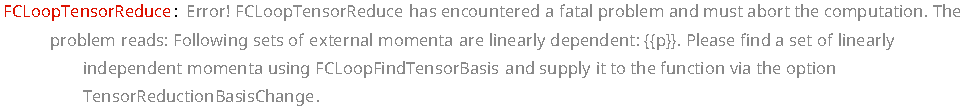
\includegraphics[width=0.6\linewidth]{img/01k9v9jxkacva.pdf}
\end{figure}
\FloatBarrier

\begin{dmath*}\breakingcomma
\text{\$Aborted}
\end{dmath*}

Using \texttt{FCLoopFindTensorBasis} we can construct an alternative
basis and supply it to the reduction procedure. In this case we need to
introduce an auxiliary vector \texttt{n}. For simplicity, we choose it
to be light-like

\begin{Shaded}
\begin{Highlighting}[]
\NormalTok{FCLoopFindTensorBasis}\OperatorTok{[\{}\FunctionTok{p}\OperatorTok{\},} \OperatorTok{\{\},} \FunctionTok{n}\OperatorTok{]}
\end{Highlighting}
\end{Shaded}

\begin{dmath*}\breakingcomma
\{\{p,n\},\{\},\{\}\}
\end{dmath*}

In this case to complete the reduction we need to use IBPs. Furthermore,
the existing topology should be augmented to include the new auxiliary
vector.

\begin{Shaded}
\begin{Highlighting}[]
\NormalTok{amp3red }\ExtensionTok{=}\NormalTok{ FCLoopTensorReduce}\OperatorTok{[}\NormalTok{amp3}\OperatorTok{,} \OperatorTok{\{}\NormalTok{topo3}\OperatorTok{\},}\NormalTok{ TensorReductionBasisChange }\OtherTok{{-}\textgreater{}} \OperatorTok{\{\{}\FunctionTok{p}\OperatorTok{\}} \OtherTok{{-}\textgreater{}} \OperatorTok{\{}\FunctionTok{p}\OperatorTok{,} \FunctionTok{n}\OperatorTok{\}\},}\NormalTok{ AuxiliaryMomenta }\OtherTok{{-}\textgreater{}} \OperatorTok{\{}\FunctionTok{n}\OperatorTok{\},} 
\NormalTok{   FinalSubstitutions }\OtherTok{{-}\textgreater{}} \OperatorTok{\{}\NormalTok{SPD}\OperatorTok{[}\FunctionTok{n}\OperatorTok{]} \OtherTok{{-}\textgreater{}} \DecValTok{0}\OperatorTok{\}]}
\end{Highlighting}
\end{Shaded}

\begin{dmath*}\breakingcomma
\text{FCGV}(\text{GLIProduct})\left(\frac{1}{(2-D) (n\cdot p)^2}\left((\text{q1}\cdot \;\text{q2}) \left(-\gamma ^{\text{\$AL}(\text{\$58})}.\gamma ^{\mu }.\gamma ^{\text{\$AL}(\text{\$58})}\right) (n\cdot p)^2+(n\cdot p) (n\cdot \;\text{q2}) (p\cdot \;\text{q1}) \gamma ^{\text{\$AL}(\text{\$58})}.\gamma ^{\mu }.\gamma ^{\text{\$AL}(\text{\$58})}+(n\cdot p) (n\cdot \;\text{q1}) (p\cdot \;\text{q2}) \gamma ^{\text{\$AL}(\text{\$58})}.\gamma ^{\mu }.\gamma ^{\text{\$AL}(\text{\$58})}-D (n\cdot \;\text{q1}) (n\cdot \;\text{q2}) (\gamma \cdot p).\gamma ^{\mu }.(\gamma \cdot p)-D (n\cdot \;\text{q2}) (p\cdot \;\text{q1}) (\gamma \cdot n).\gamma ^{\mu }.(\gamma \cdot p)-D (n\cdot \;\text{q1}) (p\cdot \;\text{q2}) (\gamma \cdot p).\gamma ^{\mu }.(\gamma \cdot n)-D (p\cdot \;\text{q1}) (p\cdot \;\text{q2}) (\gamma \cdot n).\gamma ^{\mu }.(\gamma \cdot n)+(n\cdot p) (\text{q1}\cdot \;\text{q2}) (\gamma \cdot n).\gamma ^{\mu }.(\gamma \cdot p)+(n\cdot p) (\text{q1}\cdot \;\text{q2}) (\gamma \cdot p).\gamma ^{\mu }.(\gamma \cdot n)+2 (n\cdot \;\text{q1}) (n\cdot \;\text{q2}) (\gamma \cdot p).\gamma ^{\mu }.(\gamma \cdot p)+(n\cdot \;\text{q2}) (p\cdot \;\text{q1}) (\gamma \cdot n).\gamma ^{\mu }.(\gamma \cdot p)-(n\cdot \;\text{q2}) (p\cdot \;\text{q1}) (\gamma \cdot p).\gamma ^{\mu }.(\gamma \cdot n)-(n\cdot \;\text{q1}) (p\cdot \;\text{q2}) (\gamma \cdot n).\gamma ^{\mu }.(\gamma \cdot p)+(n\cdot \;\text{q1}) (p\cdot \;\text{q2}) (\gamma \cdot p).\gamma ^{\mu }.(\gamma \cdot n)+2 (p\cdot \;\text{q1}) (p\cdot \;\text{q2}) (\gamma \cdot n).\gamma ^{\mu }.(\gamma \cdot n)\right),G^{\text{prop2L}}(1,1,1,1,1) \;\text{FCGV}(\text{AddPropagators})(\{n\})\right)
\end{dmath*}

\begin{Shaded}
\begin{Highlighting}[]
\OperatorTok{\{}\NormalTok{newtopo}\OperatorTok{,}\NormalTok{ gliRule}\OperatorTok{\}} \ExtensionTok{=}\NormalTok{ FCLoopAugmentTopology}\OperatorTok{[}\NormalTok{topo3}\OperatorTok{,} \OperatorTok{\{}\NormalTok{SFAD}\OperatorTok{[\{\{}\DecValTok{0}\OperatorTok{,}\NormalTok{ q1 . }\FunctionTok{n}\OperatorTok{\}\}],}\NormalTok{ SFAD}\OperatorTok{[\{\{}\DecValTok{0}\OperatorTok{,}\NormalTok{ q2 . }\FunctionTok{n}\OperatorTok{\}\}]\}]}
\end{Highlighting}
\end{Shaded}

\begin{dmath*}\breakingcomma
\left\{\text{FCTopology}\left(\text{prop2LA},\left\{\frac{1}{(\text{q1}^2-m^2+i \eta )},\frac{1}{(\text{q2}^2-m^2+i \eta )},\frac{1}{((\text{q1}-\text{q2})^2+i \eta )},\frac{1}{((\text{q1}-p)^2+i \eta )},\frac{1}{((\text{q2}-p)^2+i \eta )},\frac{1}{(n\cdot \;\text{q1}+i \eta )},\frac{1}{(n\cdot \;\text{q2}+i \eta )}\right\},\{\text{q1},\text{q2}\},\{p,n\},\{\},\{\}\right),\text{FCGV}(\text{AddPropagators})(\{n\}) G^{\text{prop2L}}(\text{n1$\_$},\text{n2$\_$},\text{n3$\_$},\text{n4$\_$},\text{n5$\_$}):\to G^{\text{prop2LA}}(\text{n1},\text{n2},\text{n3},\text{n4},\text{n5},0,0)\right\}
\end{dmath*}

In this form the expression can be converted into \texttt{GLI}s and
passed to an IBP reduction tool

\begin{Shaded}
\begin{Highlighting}[]
\NormalTok{amp3red }\OtherTok{/.}\NormalTok{ gliRule}
\end{Highlighting}
\end{Shaded}

\begin{dmath*}\breakingcomma
\text{FCGV}(\text{GLIProduct})\left(\frac{1}{(2-D) (n\cdot p)^2}\left((\text{q1}\cdot \;\text{q2}) \left(-\gamma ^{\text{\$AL}(\text{\$58})}.\gamma ^{\mu }.\gamma ^{\text{\$AL}(\text{\$58})}\right) (n\cdot p)^2+(n\cdot p) (n\cdot \;\text{q2}) (p\cdot \;\text{q1}) \gamma ^{\text{\$AL}(\text{\$58})}.\gamma ^{\mu }.\gamma ^{\text{\$AL}(\text{\$58})}+(n\cdot p) (n\cdot \;\text{q1}) (p\cdot \;\text{q2}) \gamma ^{\text{\$AL}(\text{\$58})}.\gamma ^{\mu }.\gamma ^{\text{\$AL}(\text{\$58})}-D (n\cdot \;\text{q1}) (n\cdot \;\text{q2}) (\gamma \cdot p).\gamma ^{\mu }.(\gamma \cdot p)-D (n\cdot \;\text{q2}) (p\cdot \;\text{q1}) (\gamma \cdot n).\gamma ^{\mu }.(\gamma \cdot p)-D (n\cdot \;\text{q1}) (p\cdot \;\text{q2}) (\gamma \cdot p).\gamma ^{\mu }.(\gamma \cdot n)-D (p\cdot \;\text{q1}) (p\cdot \;\text{q2}) (\gamma \cdot n).\gamma ^{\mu }.(\gamma \cdot n)+(n\cdot p) (\text{q1}\cdot \;\text{q2}) (\gamma \cdot n).\gamma ^{\mu }.(\gamma \cdot p)+(n\cdot p) (\text{q1}\cdot \;\text{q2}) (\gamma \cdot p).\gamma ^{\mu }.(\gamma \cdot n)+2 (n\cdot \;\text{q1}) (n\cdot \;\text{q2}) (\gamma \cdot p).\gamma ^{\mu }.(\gamma \cdot p)+(n\cdot \;\text{q2}) (p\cdot \;\text{q1}) (\gamma \cdot n).\gamma ^{\mu }.(\gamma \cdot p)-(n\cdot \;\text{q2}) (p\cdot \;\text{q1}) (\gamma \cdot p).\gamma ^{\mu }.(\gamma \cdot n)-(n\cdot \;\text{q1}) (p\cdot \;\text{q2}) (\gamma \cdot n).\gamma ^{\mu }.(\gamma \cdot p)+(n\cdot \;\text{q1}) (p\cdot \;\text{q2}) (\gamma \cdot p).\gamma ^{\mu }.(\gamma \cdot n)+2 (p\cdot \;\text{q1}) (p\cdot \;\text{q2}) (\gamma \cdot n).\gamma ^{\mu }.(\gamma \cdot n)\right),G^{\text{prop2LA}}(1,1,1,1,1,0,0)\right)
\end{dmath*}

Not all cases of zero Gram determinants require an auxiliary vector. If
the new basis can be constructed from a subset of the present external
momenta, this should be sufficient for the reduction. Consider e.g.~this
threshold kinematics

\begin{Shaded}
\begin{Highlighting}[]
\NormalTok{FCClearScalarProducts}\OperatorTok{[]}
\NormalTok{SPD}\OperatorTok{[}\NormalTok{p1}\OperatorTok{]} \ExtensionTok{=}\NormalTok{ mm;}
\NormalTok{SPD}\OperatorTok{[}\NormalTok{p2}\OperatorTok{]} \ExtensionTok{=}\NormalTok{ mm;}
\NormalTok{SPD}\OperatorTok{[}\NormalTok{p1}\OperatorTok{,}\NormalTok{ p2}\OperatorTok{]} \ExtensionTok{=}\NormalTok{ mm;}
\end{Highlighting}
\end{Shaded}

\begin{Shaded}
\begin{Highlighting}[]
\NormalTok{topo4 }\ExtensionTok{=}\NormalTok{ FCTopology}\OperatorTok{[}\StringTok{"tri1l"}\OperatorTok{,} \OperatorTok{\{}\NormalTok{SFAD}\OperatorTok{[\{}\FunctionTok{q}\OperatorTok{,} \FunctionTok{m}\SpecialCharTok{\^{}}\DecValTok{2}\OperatorTok{\}],}\NormalTok{ SFAD}\OperatorTok{[\{}\FunctionTok{q} \SpecialCharTok{{-}}\NormalTok{ p1}\OperatorTok{,} \DecValTok{0}\OperatorTok{\}],}\NormalTok{ SFAD}\OperatorTok{[\{}\FunctionTok{q} \SpecialCharTok{{-}}\NormalTok{ p2}\OperatorTok{,} \DecValTok{0}\OperatorTok{\}]\},} \OperatorTok{\{}\FunctionTok{q}\OperatorTok{\},} \OperatorTok{\{}\NormalTok{p1}\OperatorTok{,}\NormalTok{ p2}\OperatorTok{\},} \OperatorTok{\{\},} \OperatorTok{\{\}]}
\end{Highlighting}
\end{Shaded}

\begin{dmath*}\breakingcomma
\text{FCTopology}\left(\text{tri1l},\left\{\frac{1}{(q^2-m^2+i \eta )},\frac{1}{((q-\text{p1})^2+i \eta )},\frac{1}{((q-\text{p2})^2+i \eta )}\right\},\{q\},\{\text{p1},\text{p2}\},\{\},\{\}\right)
\end{dmath*}

\begin{Shaded}
\begin{Highlighting}[]
\NormalTok{amp4 }\ExtensionTok{=}\NormalTok{ FCGV}\OperatorTok{[}\StringTok{"GLIProduct"}\OperatorTok{][}\NormalTok{GSD}\OperatorTok{[}\FunctionTok{q}\OperatorTok{]}\NormalTok{ . GAD}\OperatorTok{[}\SpecialCharTok{\textbackslash{}}\OperatorTok{[}\NormalTok{Mu}\OperatorTok{]]}\NormalTok{ . GSD}\OperatorTok{[}\FunctionTok{r}\OperatorTok{],}\NormalTok{ GLI}\OperatorTok{[}\StringTok{"tri1l"}\OperatorTok{,} \OperatorTok{\{}\DecValTok{1}\OperatorTok{,} \DecValTok{1}\OperatorTok{,} \DecValTok{1}\OperatorTok{\}]]}
\end{Highlighting}
\end{Shaded}

\begin{dmath*}\breakingcomma
\text{FCGV}(\text{GLIProduct})\left((\gamma \cdot q).\gamma ^{\mu }.(\gamma \cdot r),G^{\text{tri1l}}(1,1,1)\right)
\end{dmath*}

\begin{Shaded}
\begin{Highlighting}[]
\NormalTok{FCLoopTensorReduce}\OperatorTok{[}\NormalTok{amp4}\OperatorTok{,} \OperatorTok{\{}\NormalTok{topo4}\OperatorTok{\}]}
\end{Highlighting}
\end{Shaded}

\FloatBarrier
\begin{figure}[!ht]
\centering
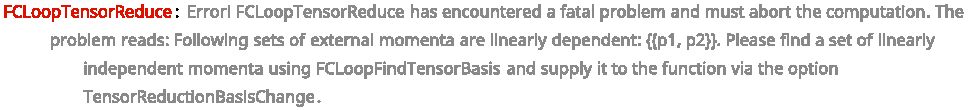
\includegraphics[width=0.6\linewidth]{img/1stlzmp72npin.pdf}
\end{figure}
\FloatBarrier

\begin{dmath*}\breakingcomma
\text{\$Aborted}
\end{dmath*}

\begin{Shaded}
\begin{Highlighting}[]
\NormalTok{FCLoopFindTensorBasis}\OperatorTok{[\{}\NormalTok{p1}\OperatorTok{,}\NormalTok{ p2}\OperatorTok{\},} \OperatorTok{\{\},} \FunctionTok{n}\OperatorTok{]}
\end{Highlighting}
\end{Shaded}

\begin{dmath*}\breakingcomma
\left(
\begin{array}{c}
 \;\text{p1} \\
 \;\text{p2} \\
 \;\text{p2}\to \;\text{p1} \;\text{FCGV}(\text{Prefactor})(1) \\
\end{array}
\right)
\end{dmath*}

Here the momenta p1 and p2 are obviously identical, so we need to do the
reduction w.r.t p1 only

\begin{Shaded}
\begin{Highlighting}[]
\NormalTok{FCLoopTensorReduce}\OperatorTok{[}\NormalTok{amp4}\OperatorTok{,} \OperatorTok{\{}\NormalTok{topo4}\OperatorTok{\},}\NormalTok{ TensorReductionBasisChange }\OtherTok{{-}\textgreater{}} \OperatorTok{\{\{}\NormalTok{p1}\OperatorTok{,}\NormalTok{ p2}\OperatorTok{\}} \OtherTok{{-}\textgreater{}} \OperatorTok{\{}\NormalTok{p1}\OperatorTok{\}\}]}
\end{Highlighting}
\end{Shaded}

\begin{dmath*}\breakingcomma
\text{FCGV}(\text{GLIProduct})\left(\frac{(\text{p1}\cdot q) (\gamma \cdot \;\text{p1}).\gamma ^{\mu }.(\gamma \cdot r)}{\text{mm}},G^{\text{tri1l}}(1,1,1)\right)
\end{dmath*}
\end{document}
